\chapter{Event Spotting on Video}
\label{chap:event}

\section{Introduction}
As mentioned in chapter \ref{chap:intro}, our ultimate aim was to find all the events in the search video $(\mathcal{V})$ which are similar to the event in given query $(\mathcal{Q})$  for a given video ($\mathcal{V}$) and a query $(\mathcal{Q})$. Since video is temporal sequence we have to model temporal dependencies
in the data at sub-event level. 

\textit{Dynamic Time Warping (DTW)} is well known for it's ability to compare two time dependent sequences. Intuitively, the sequences are warped in a nonlinear fashion to match each other. Even though DTW was developed for compare different speech patterns in ASR (Automatic Speech Recognition), nowadays DTW has been applied to other fields \cite{muller2007information}.  So we decided to make use of DTW for comparing (and hence spotting events) in Query and Search Video.

Now we have to extract effective features from video sequence so that features will be able to describe events  in video. We decided to make use of Deep Neural Network for extracting these features. 

In this chapter, We will fist discuss why we preferred  DNN over classical feature extractors. In Section \ref{sec:event:unsupervised}, we go through different unsupervised methods attempted to answer the question \textit{``Will any unsupervised Deep Learning Techniques work for feature extraction ?"}. Later in section \ref{sec:event:supervised}, we go through experiments which uses supervised CNNs  

\section{Why Deep Neural Networks?}
\label{sec:event:why}
We have to capture underlying temporal structures of actions (i.e. intra-dependencies) through feature representations. Some of classical features in videos are SIFT(Scale-invariant feature transform), HOG (Histogram of oriented gradients), Optical Flow, HOF (Histograms of flow orientations), HOG3D (Histograms of 3D gradients), MBH (motion boundary histograms). These classical feature extraction requires high amount of computaion \cite{baker2011database,chatfield2011devil}. This time-consuming process of feature extraction limits the speed of testing and hence limiting the scope of real time applications.

In recent years, deep learning has produced remarkable results and significantly outperformed state-of-the-art the classical methods \cite{KarpathyCVPR14}. Deep Neural Networks (DNNs) is able to learning the feature representation directly from input and hence bring significant performance boosting (refer chapter \ref{chap:dnn}). Moreover, bottleneck features generated from deep neural networks (Deep Bottleneck Features) are found as better features in automatic speech recognition (ASR) systems \cite{yu2011improved,gehring2013extracting}.

\section{Unsupervised Methods}
\label{sec:event:unsupervised}
Our initial approach was to find out \textit{``Will any unsupervised Deep Learning Techniques work for feature extraction ?"}. Experiments are done on the \textbf{OSUPEL basketball dataset} \cite{brendel2011probabilistic}.The OSUPEL basketball dataset contains videos of drills and small basketball games. Since these videos were shot in a real-world setting it contains challenges like slow and sudden camera motion, motion blur of fast actions, inter-player occlusions, and varying illumination. Resolution of data set is $960 \times 540$ pixels and frame rate is $29$fps.

In this section we go through different unsupervised Deep Neural Network methods that has been experimented. 

\subsection{Deep Belief Network} 
We took complete video and reduced resolution to $256 \times 144$ pixels (from $960 \times 540$). Then each frame is fed to a \textit{Deep Belief Network (DBN)} which tries to reduce it's dimensionality. Different DBNs with different sizes of deep bottleneck features (400,1000 and 2000) were analysed. But we encountered a problem: the features we obtained were somewhat random. We found that the large size of the weight matrix is the reason behind this issue. To train such a big network, we need a big data-set.

\subsection{DBN on DCT Coefficients}
Since our previous attempt failed as the input dimension was too big, we decided to make use of Discrete Cosine Transform (DCT).Advantage of DCT can be implemented using a fast algorithm and is commonly used for dimensionality reduction in images/videos \cite{er2005high}. Reduced resolution video ($256 \times 144$) is taken and DCT is computed for each frame. The low-frequency coefficients of DCT is taken (top 1500) and is normalised with respect to mean. Then we used Deep Belief Network which tries to reduce dimensionality (to 400/200).

But it was found that DBN features yields same outputs, irrespective of the input, if we use more than one layer. With a single layer Restricted Boltzmann machine (first Layer is Gaussian-Bernoulli layer), we are getting some variation but not enough for identifying the events.\\


\begin{figure}
        \centering
        \begin{subfigure}[b]{\textwidth}
        			\centering
                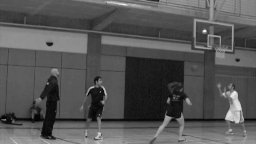
\includegraphics[scale=1]{./imgs/Original.png}
                \caption{Original frame}
                \label{fig:original}
        \end{subfigure}%
        %newline
        
        \begin{subfigure}[b]{0.45\textwidth}
        		\centering
        		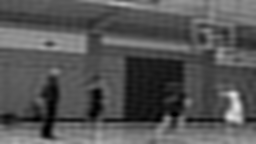
\includegraphics[scale=1]{./imgs/DCT.png}
        		\caption{Reconstructed frame from top 1500 DCT coefficients}
        		\label{fig:dct}
        \end{subfigure}
        ~%~ %add desired spacing between images, e. g. ~, \quad, \qquad, \hfill etc.
        \begin{subfigure}[b]{0.45\textwidth}
        			\centering
                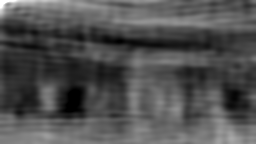
\includegraphics[scale=1]{./imgs/DBN.png}
                \caption{Reconstructed frame from DBN features (single layer)}
                \label{fig:dbn}
        \end{subfigure}
        \caption{ A Analysis of DBN features}
        \label{fig:dct+dbn}
\end{figure}.

\subsection{SdA on DCT Coefficients}
Instead of using DBN to reduce the dimensionality, we tried to use \textit{Stacked Denoising Auto-encoder (SdA)} for same. It also failed to capture features which are abstract representation of events in the video.\\
Since SdA tries to learn weights so that reconstruction error is less and most of DCT low frequency Coefficients across frames having less variance, SdA tries to learn common features instead of varying features.\\

\subsection{Using DCT and GMM}
\label{sec:event:dct_gmm}
This section discuss a combined approach which uses principles of Gaussian posteriorgram and Vector Space Model.

The concept of the Gaussian posteriorgram is similar to the posterior feature vectors\citep{zhang2010towards}. For each frame, a probability vector containing the posterior probabilities of each of the Gaussian components in a Gausian Mixture Model is computed. This probability vector is called as  Gaussian posteriorgram. 

Vector Space Model (VSM) is widely used NLP for Information retrieval. The Vector Space Model has proved to be successful for many image applications such as classification and video indexing and retrieval \citep{galmar2007analysis}. 

We build smaller GMMs (4 - 50 mixtures), and trained them with some of the videos. Then responsibility of each frame in the search and query video is calculated. We assume the query contains only one event, so we represented each query as a single vector (mean of the responsibilities of all frames in the query). Inner product of each search video vector (corresponding to each frame of the search video) with representative vector of query video is taken. Finally, all the continuous frames of length at-least half of that of the query with all inner products greater than a threshold, are considered similar events. With 5 mixtures and 0.65 as the threshold, we captured most events but also captured a lot of false positives.

\section{Supervised Methods}
\label{sec:event:supervised}
Through the experiments mentioned in section  \ref{sec:event:unsupervised}, we found that deep bottleneck features using unsupervised learning does not gives any benefit in identification of events in Video. Moreover, these techniques tries to capture more similar features in video, rather than capturing abstract representations which describes events in video.

In this section we examines use Convolutional Neural Networks for extracting deep bottleneck features. CNNs has produced many ground breaking results in many on various research topics of image and video processing \citep{KarpathyCVPR14, ji20133d, krizhevsky2012imagenet}. 

Experiments described in this section are done on the \textbf{OSUPEL basketball dataset} \cite{brendel2011probabilistic} (hereafter refereed as basketball dataset) and \textbf{Microsoft Research Action Dataset \RN{2}} (hereafter refereed as MSR dataset). MSR dataset contains of 54 videos recorded in a crowded environment. These videos has  a resolution of $320\times240$ pixels and frame rate of $15$ fps. There are three action types in this dataset: \textit{hand waving, handclapping, and boxing } and multiple actions are present in each video.

\subsection{3D-CNN with color map feature}
For extracting deep bottleneck features, we can use 3D-CNN model. This model tries extracts features from both spatial and temporal dimensions by performing three Dimensional convolutions, thereby capturing the motion information encoded in adjacent frames\citep{ji20133d}.

Videos of reduced resolution is fed into 3D-CNN model with 3 color channel (RGB) as input feature maps. 

In case of basketball dataset, input is size of $144 \times 256 \times 5 \times 3$ (5 in time axis). And for MSR dataset size of input is $120 \times 160 \times 5 \times 3$

Classification result of 3d-CNN was biased on both datasets, Almost all of data was classified into a single class. Even though we repeated experiment by varying input and kernel dimension, we got same result. Also result of the same experiment on reduced dataset (removed some of the classes), had same bias. 

\subsection{CNN with color map feature}
\citet{KarpathyCVPR14} showed that single-frame architecture with color map as input will produce satisfactory results. So each frame of videos with reduced resolution is fed into CNN model with 3 color channel (RGB) as input feature maps.

In case of basketball dataset, input is size of $X \times Y \times 3$. Using shorthand notation, the full architecture is $C(15, 15, 10)-P(4, 4)-C(5, 5, 10)-P(2, 2)-FC(500)$. $C(X, Y, K)$ denotes convolutional layer with $K$ kernels of size $X \times Y$. Max-Pooling layer of size $X \times Y$ is represented as $P(X,Y)$. $FC(N)$ represents a fully connected layer with $N$ nodes. 

For MSR dataset size of input is $X \times Y \times 3$. The full architecture of CNN is $C(10, 10, 7)-P(2, 2)-C(5, 5, 5)-P(2, 2)-FC(100)$

The result of Experiments is shown in table \ref{table:cnn_res}.

We found that CNN with single frame will give better classification accuracy than 3D-CNN. We belief that it may be due to deficiency of data (3D-CNN has only $1/5^{th}$ of data point when compared to single frame CNN).

Even though, MSR Dataset has produced good result, result of basketball dataset is poor. The reason behind this lies in the fact that basketball dataset has more camera motion, motion blur and scaling compared to MSR dataset.

\begin{table}[h]
\centering
\begin{tabular}{|l|c|c|}
\hline
Method & OSUPEL Basketball& MSR Action\\
       & Dataset          &Dataset \\
\hline
\hline
3D-CNN  &24.769\%   &39.063\% \\
\hline
CNN with color map  &69.375\%   &85.687\% \\
\hline
CNN with frame-difference &&\\
and edge detection &84.219\%   &91.508\% \\
\hline
HOG-MHI+Hierarchical &&\\
Motion Filter  & -  &78.8\% \\
\hline
 &&\\
 & 79.98\%   & - \\
\hline  
\end{tabular}
\caption[Classification Accuracy]{Classification Accuracy}
\label{table:cnn_res}
\end{table} 

\subsection{CNN with frame-difference and edge detection}

Many have attempted to give some pre-processed input to Convolutional Neural Networks and able to produce exceptional result in video event recognition \citep{ji20133d}. So instead of giving 3 colour maps, a pre-processed input is fed to 2D CNN.

For each frame (of reduced resolution video), frame differencing and edge detection is performed. The frame differencing will act as background subtraction. The Edges of images is found with Canny edge detection algorithm. A gray scale copy of Original frame is also kept. Thus CNN takes 3 feature maps:
\begin{enumerate}
\item Gray scale frame.
\item Edge (using Canny edge detection).
\item Frame difference.
\end{enumerate}

The architecture of CNN is $C(11, 11, 10)-P(4, 4)-C(6, 6, 10)-P(2, 2)-FC(200)$ for basketball dataset and $C(11, 11, 10)-P(4,4)-C(5, 5, 6)-P(2,2)-FC(50)$ for MSR dataset. The result of Experiments is shown in table \ref{table:cnn_res}.

\begin{table}[h]
\centering
\begin{tabular}{|c|c|l|l|l|}
\hline
No: of &&&&\\
GMM Mixtures & Threshold & Avg. Precision & Avg. Recall & F-measure\\
\hline
\hline
 4 	&0.7 	&0.2203 	& 0.1511	&0.1792\\
 5 	&0.6 	&0.2252 	& 0.1531	&0.1823\\
 6 	&0.6 	&0.2340 	& 0.1871	&0.2080\\
 7 	&0.4 	&0.2204 	& 0.1711	&0.1926\\
 9 	&0.6 	&0.1909 	& 0.1951	&0.1930\\
10 	&0.3 	&0.2069 	& 0.2311	&\textbf{0.2183}\\
14 	&0.4 	&0.1699 	& 0.1331	&0.1492\\
\hline  
\end{tabular}
\caption[Event spotting using GMM/VSM on CNN(Gray,Frame diff,Edge) bottleneck features (MSR Action Dataset) ]{ Precision \& Recall  of GMM/VSM on CNN bottleneck features (MSR dataset)}
\label{table:cnn_gmm_res_msr}
\end{table} 

\subsubsection{GMM on bottleneck features}
Similar to the method discussed in section \ref{sec:event:dct_gmm}, we examined the performance of approach (based on principle of Gaussian posteriorgram and Vector Space Model) on deep bottleneck features extracted using above model. 

The \textit{precision, recall and F-measure} of the experiment given in table \ref{table:cnn_gmm_res_msr} (MSR dataset) and table \ref{table:cnn_gmm_res_basket} (Basketball dataset).

\begin{table}[h]
\centering
\begin{tabular}{|c|c|l|l|l|}
\hline
No: of &&&&\\
GMM Mixtures & Threshold & Avg. Precision & Avg. Recall & F-measure\\
\hline
\hline
4 	&0.7 	&0.4874 	& 0.6586	&0.5602\\
5 	&0.6 	&0.5999 	& 0.7348	&0.6605\\
6 	&0.7 	&0.6311 	& 0.7513	&0.6860\\
6 	&0.8 	&0.6469 	& 0.7501	&0.6947\\
7 	&0.6 	&0.6365 	& 0.7864	&0.7035\\
7 	&0.7 	&0.6575 	& 0.7847	&0.7155\\
8 	&0.7 	&0.7030 	& 0.7776	&0.7384\\
8 	&0.8 	&0.7194 	& 0.7754	&0.7464\\
9 	&0.7 	&0.7052 	& 0.7718	&0.7370\\
9 	&0.8 	&0.7234 	& 0.7706	&0.7462\\
10 	&0.8 	&0.7582 	& 0.7462	&0.7522\\
11 	&0.7 	&0.7898 	& 0.7669	&0.7782\\
12 	&0.7 	&0.7927 	& 0.7786	&0.7856\\
12 	&0.8 	&0.8093 	& 0.7774	&\textbf{0.7930}\\
13 	&0.7 	&0.8319 	& 0.7394	&0.7829\\
14 	&0.7 	&0.7885 	& 0.7601	&0.7740\\
14 	&0.8 	&0.8021 	& 0.7574	&0.7791\\
14 	&0.9 	&0.8173 	& 0.7574	&0.7862\\
\hline  
\end{tabular}
\caption[Event spotting using GMM/VSM on CNN(Gray,Frame diff,Edge) bottleneck features (MSR Action Dataset) ]{ Precision \& Recall  of GMM/VSM on CNN bottleneck features (Basketball dataset)}
\label{table:cnn_gmm_res_basket}
\end{table}

\subsubsection{DTW on bottleneck features}
\textit{Dynamic Time Warping (DTW)} using deep bottleneck features extracted with help of the CNN model. DTW can be used for both event classification and spotting. In classification we have template sequence for each event type, and DTW of test sequence with each of the template sequence is performed and test sequence is classified as event which had least score (normalized). In event spotting we have query sequence and we have to find events in a test, so that event's DTW score(normalized) is less than a threshold.


The \textit{True Postive \& False Postive} of the DTW event classification on basketball dataset given in table \ref{table:cnn_dtw_res_basket} and that of MSR dataset is given by \ref{table:cnn_dtw_res_msr}

\begin{table}[h]
\centering
\begin{tabular}{|l|l|l|l|}
\hline
Query Class & True Postive & False Postive & Accuracy \\ \hline
Dribbling   &265  &546   &0.3267\\
Jumping     &165  &354   &0.3179\\
Passing     &321  &768   &0.2947\\
Catching    &331  &652   &0.3367\\
Holding Ball &193  &428   &0.3108\\
\hline
Avg         &255  &549.6 &0.3174\\
\hline  
\end{tabular}
\caption[Event classification using DTW on CNN bottleneck features (OSUPEL basketball dataset) ]{True Postive \& False Positive using DTW on CNN bottle neck features (basketball dataset)}
\label{table:cnn_dtw_res_basket}
\end{table} 

\begin{table}[h]
\centering
\begin{tabular}{|l|l|l|l|}
\hline
Query Class & True Postive & False Postive & Accuracy \\ \hline
Clapping    &312	&153	&0.671\\
Hand waving &526	&387	&0.576\\
Boxing      &475	&146	&0.765\\
\hline
Avg	&437.667	&228.667	&0.671\\
\hline  
\end{tabular}
\caption[Event classification using DTW on CNN bottleneck features (MSR Action dataset \RN{2}) ]{True Postive \& False Positive using DTW on CNN bottleneck features (MSR dataset)}
\label{table:cnn_dtw_res_msr}
\end{table} 

The figure.\ref{fig:dtw} describe \textit{Target score vs Non-target} score of basketball dataset and MSR dataset. From the graph we can understand that by using DTW on bottleneck features we cannot perform event spotting.

\section{Summary}

TODO .............